%********************************************************************
% Appendix
%*******************************************************
% If problems with the headers: get headings in appendix etc. right
\markboth{\spacedlowsmallcaps{Appendix}}{\spacedlowsmallcaps{Appendix}}
%************************************************
\chapter{Appendix: Preliminary Results on Other Gradient Estimators}\label{chap:appendix}

\section{Half-Cheetah Mujoco Task}
\vspace{-0.05in}
Here we present all the exploratory results for the two versions introduced in section \ref{subsec:oge} for what concert the Half-Cheetah task.
\begin{figure*}[h]
	\begin{minipage}[h]{1\textwidth}
		\centering
		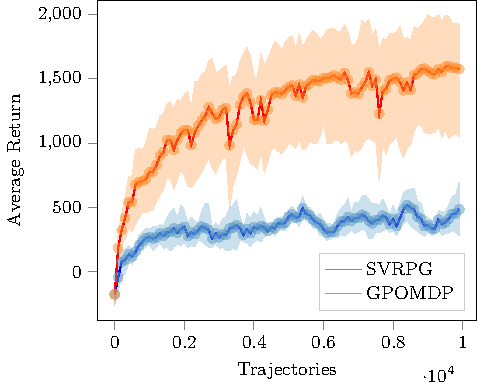
\includegraphics[width=0.75\textwidth]{Images/Experiments/half_cheetah_GPOMDP_vs_NonSelf_SVRPG_B.pdf}
		\vspace{-0.1in}
		\caption{On-line performance over sampled trajectories of \acs{SVRPG} vs G(PO)MDP in the Half-Cheetah task where we used \ref{E:svrpg.b.version} as gradient estimator, with 90\% confidence intervals.}
		\label{fig:hctwo}
	\end{minipage}
	\vspace{-0.15in}
\end{figure*}
\begin{figure*}[h]
	\begin{minipage}[h]{1\textwidth}
		\centering
		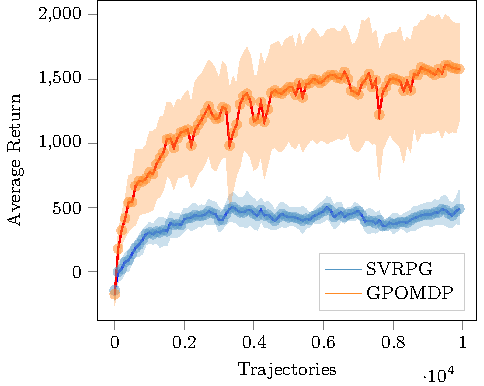
\includegraphics[width=0.75\textwidth]{Images/Experiments/half_cheetah_GPOMDP_vs_NonSelf_SVRPG_C.pdf}
		\vspace{-0.1in}
		\caption{On-line performance over sampled trajectories of \acs{SVRPG} vs G(PO)MDP in the Half-Cheetah task where we used \ref{E:svrpg.c.version} as gradient estimator, with 90\% confidence intervals.}
		\label{fig:hctwo}
	\end{minipage}
	\vspace{-0.15in}
\end{figure*}

\begin{figure*}[h]
	\begin{minipage}[h]{1\textwidth}
		\centering
		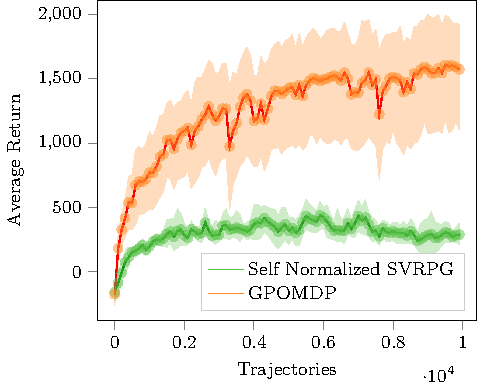
\includegraphics[width=0.75\textwidth]{Images/Experiments/half_cheetah_GPOMDP_vs_SN_SVRPG_B.pdf}
		\vspace{-0.1in}
		\caption{On-line performance over sampled trajectories of Self Normalized \acs{SVRPG} vs G(PO)MDP in the Half-Cheetah task where we used \ref{E:svrpg.b.version} as gradient estimator, with 90\% confidence intervals.}
		\label{fig:hctwo}
	\end{minipage}
	\vspace{-0.15in}
\end{figure*}
\begin{figure*}[h]
	\begin{minipage}[h]{1\textwidth}
		\centering
		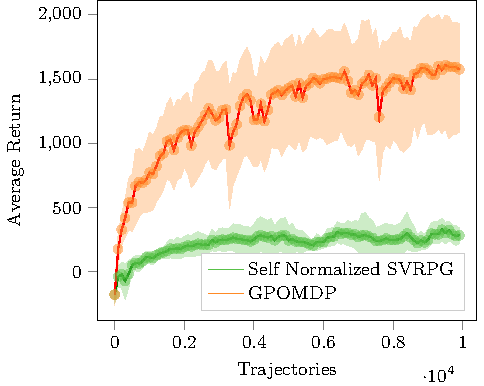
\includegraphics[width=0.75\textwidth]{Images/Experiments/half_cheetah_GPOMDP_vs_SN_SVRPG_C.pdf}
		\vspace{-0.1in}
		\caption{On-line performance over sampled trajectories of Self Normalized \acs{SVRPG} vs G(PO)MDP in the Half-Cheetah task where we used \ref{E:svrpg.c.version} as gradient estimator, with 90\% confidence intervals.}
		\label{fig:hctwo}
	\end{minipage}
	\vspace{-0.15in}
\end{figure*}


\begin{figure*}[h]
	\begin{minipage}[h]{1\textwidth}
		\centering
		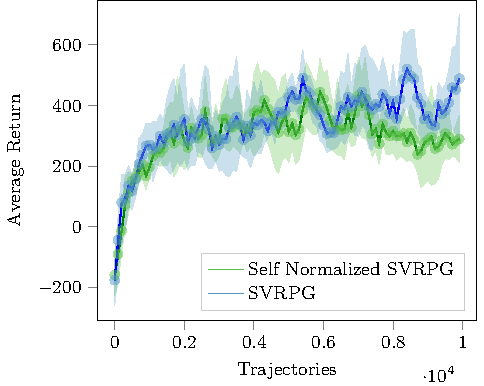
\includegraphics[width=0.75\textwidth]{Images/Experiments/half_cheetah_SVRPG_vs_SN_SVRPG_B.pdf}
		\vspace{-0.1in}
		\caption{On-line performance over sampled trajectories of Self Normalized \acs{SVRPG} vs \acs{SVRPG} in the Half-Cheetah task where we used \ref{E:svrpg.b.version} as gradient estimator, with 90\% confidence intervals.}
		\label{fig:hctwo}
	\end{minipage}
	\vspace{-0.15in}
\end{figure*}
\begin{figure*}[h]
	\begin{minipage}[h]{1\textwidth}
		\centering
		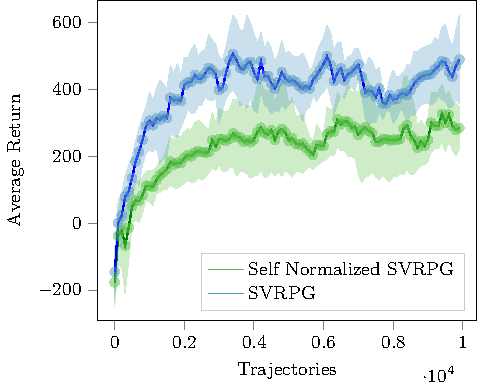
\includegraphics[width=0.75\textwidth]{Images/Experiments/half_cheetah_SVRPG_vs_SN_SVRPG_C.pdf}
		\vspace{-0.1in}
		\caption{On-line performance over sampled trajectories of Self Normalized \acs{SVRPG} vs \acs{SVRPG} in the Half-Cheetah task where we used \ref{E:svrpg.c.version} as gradient estimator, with 90\% confidence intervals.}
		\label{fig:hctwo}
	\end{minipage}
	\vspace{-0.15in}
\end{figure*}

\clearpage
\section{Swimmer Mujoco Task}
\vspace{-0.05in}
Here we present all the exploratory results for the two versions introduced in section \ref{subsec:oge} for what concert the Swimmer task.
\begin{figure*}[h]
	\begin{minipage}[h]{1\textwidth}
		\centering
		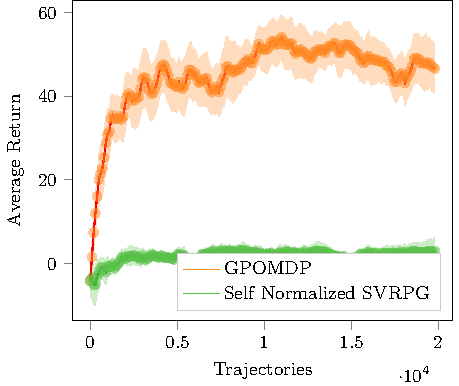
\includegraphics[width=0.75\textwidth]{Images/Experiments/swimmer_Self_SVRPG_vs_GPOMDP_B.pdf}
		\vspace{-0.1in}
		\caption{On-line performance over sampled trajectories of Self Normalized \acs{SVRPG} vs G(PO)MDP in the Swimmer task where we used \ref{E:svrpg.b.version} as gradient estimator, with 90\% confidence intervals.}
		\label{fig:hctwo}
	\end{minipage}
	\vspace{-0.15in}
\end{figure*}
\begin{figure*}[h]
	\begin{minipage}[h]{1\textwidth}
		\centering
		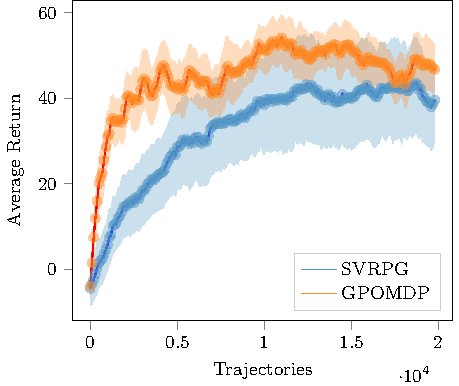
\includegraphics[width=0.75\textwidth]{Images/Experiments/swimmer_SVRPG_vs_GPOMDP_B.pdf}
		\vspace{-0.1in}
		\caption{On-line performance over sampled trajectories of \acs{SVRPG} vs G(PO)MDP in the Swimmer task where we used \ref{E:svrpg.b.version} as gradient estimator, with 90\% confidence intervals.}
		\label{fig:hctwo}
	\end{minipage}
	\vspace{-0.15in}
\end{figure*}